
\chapter{II. Courants, sensibilités, figures de l’islam de France (i)
}

\mn{LUNDI 22 NOVEMBRE 2021 (2e
cours)}


% ------------------------------------------------------------

\section{Les premières associations cultuelles (FNMF, RMF, GIF, UOIF, FNGMP,
FFAIACCA…)}

\subsection{Introduction}

\paragraph{Description de l'islam consulaire}

\begin{figure}
    \centering
        \sidecaption{Algérie : un acteur historique}
    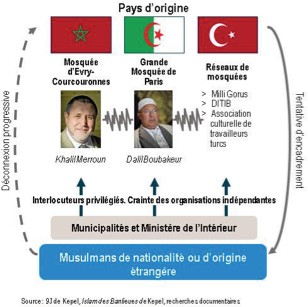
\includegraphics[width=\textwidth]{ImageIslamFrance/media/image7.jpeg}

    \label{fig:my_label}
\end{figure}


\subsection{FNGMP - Fédération Nationale de la Grande Mosquée de Paris - Algérie}

un réseau qui s'est constitué à partir d'Algériens travailleurs revenant en Algérie. 250 lieux de culte en France, rattachés à ce réseau. Elle ne réunit pas la totalité des mosquées de tendance algérienne.
\textbf{Daniel Boubakeur} figure charismatique qui donne l'impression d'un réseau organisé et puissant. 
Beaucoup d'algériens sont des Chibanis
\sn{ chibanis : Les chibanis, “cheveux blancs” en arabe dialectal, ce sont les vieux immigrés maghrébins. voir \url{https://www.histoire-immigration.fr/nos-ancetres-les-chibanis}}
auxquels se sont ajoutés des jeunes étudiants.

La FNGMP accueille 120 imams algériens détachés (voir p. \pageref{par:IslamConsulaireAlgérie} pour ces imams.).

A succédé le recteur Chems-eddine Hafiz, avocat, moins théologien et plus "laic" de la GMP. Il a été l'ancien avocat du Front Polisario. 


\paragraph{détail de l'islam Consulaire Algérien}



Environ la moitié des ressortissants algériens qui vivent à l'étranger
résident en France. On estime qu'environ 1,5 million des musulmans de
France sont algériens ou d'origine algérienne, ce qui en fait la
communauté la plus importante numériquement parmi les musulmans de
France. Cette importance démographique, ainsi que les liens
historiques qui unissent l'Algérie et la France, sont à l'origine de
cette volonté partagée par les deux pays de faire jouer à l'Algérie un
rôle majeur dans la gestion de l'islam en France.

L'islam consulaire algérien est apparu tardivement. En effet, dans les
années 1960 et 1970, l'Amicale des Algériens en Europe sert
principalement de \emph{« courroie de transmission entre un pouvoir
auréolé d'une indépendance fraîchement acquise et des migrants démunis
des solidarités communautaires »} ou joue un rôle
« d'interface » entre les migrants et les consulats algériens ou avec
les autorités françaises. Son rôle religieux est marginal
puisqu'elle n'a organisé la venue que de neufs imams
durant cette période, afin d'offrir une assistance spirituelle aux
Algériens émigrés. Ce n'est qu'en 1982, lorsqu'Alger reprend le
contrôle de la Grande Mosquée de Paris, que l'État algérien commence à
financer le culte musulman en France, constitue un réseau d'associations
cultuelles et construit des salles de prières.

L'accession de Cheikh Abbas au poste de recteur de la Grande Mosquée de
Paris (GMP) marque un double tournant, à la fois dans le rôle de
l'Algérie à l'égard de l'islam en France et dans celui dévolu à la
Grande Mosquée de Paris. En effet, à partir des années 1980, l'État
algérien tente de s'imposer comme le chef de file de l'islam en France.
Ce rôle sera conforté par l'action de Charles Pasqua au ministère de
l'Intérieur. Il tente d'organiser l'islam français autour de la Grande
Mosquée de Paris et du réseau associatif cultuel algérien, en octroyant
à celle-là le « monopole » de l'abattage rituel en France. La guerre
civile, la décennie noire du terrorisme du GIA et les attentats de 1995
à Paris commis par des islamistes algériens, intensifieront cette
relation entre le gouvernement français et le pouvoir algérien. La
gestion de l'islam par les réseaux algériens apparaît alors comme une
garantie face à la montée de l'islamisme politique en France, lui-même
essentiellement importé d'Algérie.

Malgré l'importance du rôle dévolu à l'islam consulaire algérien par les
pouvoirs publics, les élections successives du CFCM ont montré la
relative faiblesse des réseaux algériens auprès des musulmans de France.
La fédération nationale de la Grande Mosquée de Paris, qui rassemble
l'ensemble des associations cultuelles d'obédience algérienne, est ainsi
la grande perdante des premières élections de 2003, face à l'UOIF et à
la Fédération des Marocains de France : la nomination de Dalil
Boubakeur, recteur de la Grande Mosquée, à la tête du CFCM n'est due
qu'à l'accord passé préalablement avec Nicolas Sarkozy. Cet échec
électoral met à jour le décalage entre l'influence supposée, et
entretenue par le pourvoir public français, et celle réelle et effective
auprès des musulmans de France. Son expression la plus manifeste réside
dans le retrait de la fédération algérienne des instances du CFCM en
2008, refusant les règles du jeu démocratique et affirmant sa
prééminence sur l'islam français avec pour seuls arguments ceux du
nombre et du poids historique, avant son retour en 2012 lors de la
réforme du CFCM.

On estime aujourd'hui que la Grande Mosquée de Paris est forte d'un
réseau d'environ 250 associations et lieux de prières et qu'elle
contrôle environ 150 imams (soit 10\% environ des imams en France), dont
la majorité sont salariés
par l'Algérie (120 imams). Durant le mois du Ramadan, la France
accueille également 299 psalmodieurs et récitateurs dans le cadre
d'accords bilatéraux passés notamment avec le Royaume du Maroc et
l'Algérie. La répartition exacte de cet effectif n'est pas connue
publiquement. Ils disposent d'un visa de court séjour expirant le jour
de la fin du Ramadan et sont salariés par l'État émetteur. Malgré
un discours volontariste en matière d'accompagnement et d'encadrement de
l'islam français, notamment par sa participation à la formation des
cadres religieux aussi bien au sein de l'Institut Al-Ghazali implanté au
sein de la Grande Mosquée qu'au sein de l`université de Constantine,
l'État algérien demeure relativement en retrait. Ainsi ne participe-t-il
plus au financement du culte musulman en France qu'à hauteur de deux
millions d'euros par an environ, contre quatre millions en 2011, et près
de six millions pour le Maroc . Comme le souligne Bernard Godard,
malgré sa puissance symbolique, la Grande Mosquée de Paris joue un rôle
marginal dans l'islam français :
\begin{quote}
    \emph{« sa construction même, puis sa
gestion, en ont fait un lieu diplomatique et officiel, mais nullement un
pôle intellectuel ou proprement religieux, en dépit de la présence d'un
``Institut musulman'' »}\emph{.}
\end{quote}



% -------------------------------------------
\subsection{le FNMF et RMF : tendance Marocaine}

\begin{Synthesis}
FNMF : d'abord créé par des convertis, repris par l'islam consulaire Marocain, aspiré par le RMF.

\end{Synthesis}

  \paragraph{Le Maroc : la puissance du Rassemblement des Marocains de
  France (RMF)}


Environ un tiers des Marocains émigrés résident en France. Ils
constituent, derrière l'Algérie et son million et demi de
ressortissants, la seconde communauté musulmane française avec environ
un million de ressortissants (nationaux et binationaux). Le Maroc
s'attache à maintenir un lien avec ses ressortissants, surtout depuis
les années 1980 et 1990. Cette politique poursuit deux objectifs : l'un
économique, lié à l'importance des remises migratoires ; l'autre
sécuritaire, lié à la lutte contre l'influence de l'islamisme politique
et terroriste.

À partir des années 1960, avec l'arrivée des premières vagues de
travailleurs immigrés marocains en France, l'État chérifien a mis en
place un réseau de contrôle relativement souple, avec notamment
l'Amicale des travailleurs et commerçants marocains en France (ATCMF).
La dimension économique est ici primordiale, car la communauté marocaine
s'est structurée religieusement sans véritable appui consulaire. Les
appels répétés du roi Hassan II aux Marocains à ne pas rompre le lien
les reliant au Maroc
et à refuser l'abandon de la nationalité marocaine participent de à
cette volonté de maintenir l'effet diasporique.

Ce n'est que dans un second temps, sous l'effet de la montée de
l'islamisme au Maroc et en Europe, que le Royaume du Maroc met en place
une structure de contrôle religieux. L'État marocain va ainsi tenter de
rassembler les diverses associations musulmanes marocaines dans la
Fédération nationale des Marocains de France (FNMF)\sn{Wikipedia : La fédération nationale des musulmans de France (FNMF) est une association créée le 26 octobre 1985 par Yacoub Roty. Elle est soutenue, notamment financièrement par l'Arabie Saoudite mais est très proche du Maroc. Elle défend un islam traditionaliste.
}, transformée depuis
en Rassemblement des Marocains de France (RMF). Depuis sa création, en
1990, la Fondation Hassan II a pour but, en étroite coordination avec le
ministère des Marocains résidant à l'étranger et le ministère des
Affaires religieuses, de diffuser la culture marocaine. Forte d'un
budget annuel de 15 à 20 millions de dollars, cette organisation envoie
des imams en Europe et finance les associations cultuelles marocaines.
Dans son récent rapport relatif à l'islam en France, le Sénat estime que
le Maroc salarie actuellement 30 imams détachés. À l'occasion du
Ramadan, l'État chérifien \emph{« délègue également plus de 220 imams
par l'intermédiaire de la fondation Hassan II pour les Marocains
résidant à l'étranger »}, dont une partie en France.

Cette implication du Royaume chérifien dans la vie religieuse de ses
ressortissants est particulièrement prégnante si l'on considère le CFCM.
Par l'implantation majoritairement régionale des fidèles musulmans
d'origine marocaine et l'existence d'un réseau de mosquées dont la
surface est plus importante que celle des mosquées urbaines, la FNMF
remporte les premières élections du CFCM en 2003 ; elle devient la
principale bénéficiaire du mode de scrutin fondé sur la surface des
mosquées. Ce score fait prendre conscience aux autorités marocaines du
rôle déterminant qu'elles peuvent jouer dans l'islam français. Afin de
renforcer son poids dans l'instance représentative, le royaume du Maroc
fond la FNMF en une seule structure destinée à embrasser plus largement
encore l'ensemble des sensibilités des Marocains de France : le
Rassemblement des marocains de France (RMF).Cette politique volontariste
est un succès, comme le montrent les élections suivantes, que les
Français d'origine marocaine remportent largement en faisant ainsi
reculer l'UOIF. Au terme de son mandat, en 2008, Dalil Boukakeur,
recteur de la Grande Mosquée de Paris, sera ainsi remplacé par le
franco-marocain Mohammed Moussaoui.

L'implication de ressortissants d'origine marocaine dans les attentats
de Madrid en 2004 ainsi que la multiplication des actes de terrorisme
islamiste au Maroc ont conduit
son gouvernement à mener une lutte intense contre l'islamisme et le
terrorisme. C'est une véritable stratégie de contre-discours modéré que
tente de développer le Maroc en Europe, et plus particulièrement en
France. Elle passe par un contrôle accru des imams marocains présents
dans l'Hexagone, un renforcement de la présence d'imams agréés par le
gouvernement marocain, comme en témoigne l'accord passé en 2008 entre le
ministère de l'Intérieur français et le ministère des Affaires
religieuses marocains, prévoyant l'envoi de 30 imams en France, ou la
mise en place d'une offre de formation pour les apprentis-imams. Cette
politique d'encadrement religieux se double d'une politique de
financement : le Maroc participe ainsi au financement de la Grande
Mosquée de Strasbourg et finance en totalité la mosquée de
Saint-Étienne.

Au niveau européen, le Royaume chérifien crée, en 2010, un Conseil
européen des oulémas marocains, qui siège à Bruxelles. Selon Bernard
Godard, \emph{« Rabat tente d'installer en Europe une sorte de
contre-structure face à l'hyperactivité des deux ennemis principaux de
la conception chérifienne de la doctrine religieuse. Composé de
théologiens dont tous ne sont pas, loin s'en faut, des progressistes, il
doit contrebalancer une structure mise en place plus d'une décennie
auparavant par les Frères musulmans -- le Conseil européen de la fatwa
et de la recherche basé à Dublin --, mais doit aussi combattre la montée
inquiétante du salafisme qui influence les nouvelles générations en
Europe comme au Maroc}\emph{»}

\paragraph{cission de 2013} A l'intérieur de la structure RMF, bruits et cission à partir de 2013, le réseau va éclater. Il y avait une tendance proche des frères islamiques, et avec un lien plus compliqué avec le ministère des Habous marocains. UMF, Mohammed Moussaoui \sn{\url{https://fr.wikipedia.org/wiki/Mohammed_Moussaoui}}, récupère les 30 imams détachés marocains. Le RMF reste toujours présent mais n'a plus de subvention marocaine mais reste une expression de l'Islam Marocain en France, reconnu par le ministère des Habous Marocains.


L'implication de ressortissants belges et français, dont certains
étaient d'origine marocaine, dans les attentats de novembre 2015 en
France ainsi que dans celui de Bruxelles en mars 2016 incitent l'État
marocain à poursuivre sa politique religieuse afin de se prémunir de la
contamination djihadiste qui peut venir d'Europe.

L'inauguration en 2015 de l'Institut Mohammed VI à Rabat, participe
pleinement de cette dynamique de rayonnement religieux : cette
structure, accueillant des apprentis imams du Maroc, mais aussi
d'Afrique et d'Europe, a pour mission d'« \emph{enseigner aux nouvelles
générations d'imams et de mourchidates} {[}prédicatrices{]} \emph{les
valeurs de l'islam du juste milieu en vue de prémunir le Maroc contre
les velléités de l'extrémisme »} et d'assurer « la sécurité spirituelle
du Maroc \sn{Discours du roi du Maroc lors de l'inauguration de l'Institut
Mohammed VI à Rabat, le 27 mars 2015, cité par Ruth Grosrichard dans
\emph{Le Monde.}}» et par extension de la France .

% -------------------------------------------
\subsection{L'expression Turque : le CCMTF ou DITIB}

\begin{Def}[CCMTF]
le comité de coordination des musulmans turcs de France (CCMTF)
\end{Def}

Le nom est indicatif. Créé en 1986, au début de la constitution des fédérations musulmanes en France. 250 lieux de culte en France rattachés à cette fédérations.
 En 2013, Ahmet Ogras devient président du CCMTF. Il devient également vice-président, puis président en 2017, du Conseil français du culte musulman (CFCM) à la faveur de la présidence tournante pour 2 ans.
  
  
\paragraph{La Turquie : une gestion centralisée}
  



Selon les informations fournies par les consulats turcs en France, il y
aurait environ 600 000 Turcs et Français d'origine turque en France. Ils
sont principalement présents dans l'est de la France, à proximité de
l'Allemagne, principal foyer d'émigration turque, et dans le sillon
rhodanien. Si l'État turc ne s'est guère préoccupé de ses populations
immigrées avant les années 1980, il accorde un intérêt croissant au
renforcement des liens avec sa diaspora et du contrôle religieux qu'il
exerce sur elle.

Aussi, le ministère des Affaires religieuses, le Diyanet, en
collaboration avec le ministère des Affaires étrangères et le ministère
des Turcs en émigration, a mis en place l'Union turco-islamique des
Affaires religieuses (la DITIB) qu'il administre et finance. La DITIB
assure l'encadrement religieux des populations turques émigrées. Partout
où vit une minorité turque immigrée en Europe, la DITIB prend en charge
les organisations culturelles et cultuelles turques existantes ou
nouvellement créées, et assure la prise en charge du pèlerinage à la
Mecque et du rapatriement des corps pour les enterrements en Turquie. On
estime ainsi que le ministère des Affaires étrangères à Ankara contrôle
et gère plus de cinq cents lieux de culte, sur les mille mosquées et
salles de prières turques recensées en Europe. La gestion de l'islam
consulaire turc est donc beaucoup plus centralisée que celle de
l'Algérie ou du Maroc. Il y a dans chaque consulat turc un représentant
du DITIB, qui est habilité à inspecter les mosquées turques affiliées et
à contrôler les imams qui y officient. Chaque imam détaché reçoit
régulièrement « un bulletin du Diyanet », contenant notamment les
prêches du vendredi élaborés par le pouvoir central. Actuellement 151
imams détachés par l'État turc officient à temps plein : cet effectif
représente la moitié des 301 imams détachés, envoyés par les pays
étrangers, et fait de l'État turc la puissance étrangère la plus
investie dans la gestion du culte musulman en France.

Le mouvement du Millî Görüs, « Vision nationale » en turc, est le
principal concurrent du DITIB dans le contrôle religieux des émigrés
turcs. \emph{« Mélange de références proches de la mouvance des Frères
musulmans et d'exaltation de la grandeur perdue de l'Empire ottoman
»}, le Millî Görüs rassemble de fervents opposants à la laïcité turque
et de farouches partisans du port du voile pour les jeunes filles.
Implanté en France dès l'arrivée des premiers Turcs, il est à l'origine
de la construction des premières mosquées turques. Son ancrage local et
sa présence historique lui permettent de s'appuyer sur une
organisation très structurée, qui dispose notamment d'une société
immobilière gérant l'ensemble de son patrimoine, et qui dispose de son
propre pavillon en Arabie Saoudite ; ce qui lui permet d'organiser le
pèlerinage.

Depuis sa création au milieu en 1984, le Diyan a renforcé son
implantation au sein de la communauté turque. La France compte
aujourd'hui trois fédérations DITIB, une à Paris, une à Lyon et une
dernière, créée en 1997 à Strasbourg, qui gère l'islam truc dans le
Grand-Est. Cette fédération strasbourgeoise, dotée d'un budget annuel de
500 000 e en moyenne et contrôlant une soixantaine de mosquées, est
devenue en quelques années un acteur majeur de l'islam régional. \emph{«
Longtemps la DITIB est restée cantonnée aux zones rurales et aux villes
moyennes d'Alsace, tandis que Strasbourg était le terrain du Millî Görüs
côté turc (Mosquée Eyyub Sultan de la Meinau) et du Rassemblement des
musulmans de France côté marocain »}. L'accession d'un membre du
DITIB strasbourgeois à la présidence du CRCM ainsi que le développement
de projets éducatifs ambitieux (projet avorté de création d'une
université islamique et ouverture du lycée privé Yunus Emre à Strasbourg
en octobre 2015) constituent les éléments les plus visibles de cette
implantation : \emph{« Les courants islamiques turcs d'Europe ont
développé un islam social extrêmement actif. Focalisées sur le
resserrement des liens communautaires, leurs actions se développent sur
trois axes: création de mosquées, enseignement avec une réaffirmation de
valeurs traditionnalistes teintées d'ottomanisme et entraide sociale et
scolaire »}.


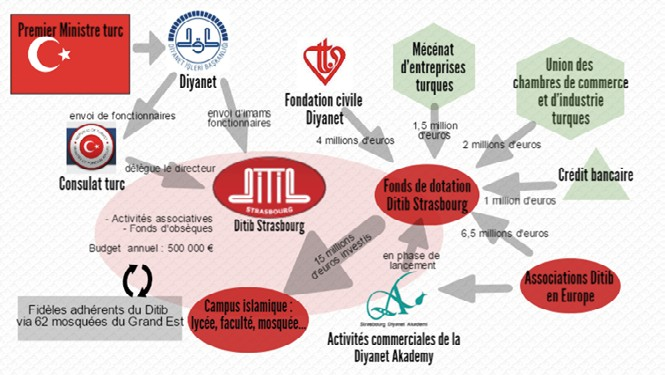
\includegraphics[width=\textwidth]{ImageIslamFrance/media/image8.jpeg}


L'islam turc ne vise pas à être hégémonique en France, mais à entretenir
l'adhésion des musulmans d'origine turque à la Turquie. Cet encadrement
très structuré, qui nourrit une vie et une pratique communautaires,
constitue à la fois un frein à l'intégration des Turcs en France mais
aussi à la propagation du salafisme parmi la communauté musulmane
d'origine turque.


% -------------------------------------------

\subsection{L'UOIF: Un islam à la française ?}
\mn{Rapport Montaigne}
 
 
 \begin{Def}[UOIF]
 L'Union des organisations islamiques de France (UOIF) est une composante
importante du paysage de l'islam français. 
 \end{Def}


\paragraph{origines-et-organisation}

Fondée en 1983 par des
étudiants tunisiens en exil, proches du Mouvement de la tendance
islamique (MTI), l'ancêtre d'Ennahda, fuyant la répression du président
Bourguiba, avait pour objectif initial de fonder une branche française
du parti islamiste tunisien. Historiquement proche des \textbf{Frères musulmans,}
dont elle constitue un acteur majeur de la branche européenne, l'UOIF,
lors de sa création, tenait un discours islamiste. Conformément à la
doctrine élaborée par Hassan Al-Banna, le fondateur du mouvement des
Frères Musulmans en 1927, les fondateurs de l'UOIF affirmaient que
l'islam est un système complet, qui concerne tous les aspects de la
vie ; il n'est donc pas seulement religieux, mais aussi politique et
social. L'objectif recherché par les Frères Musulmans est l'avènement
d'une société islamique régie par la charia.

Si ce discours islamiste est encore présent au sein de l'UOIF,
l'institutionnalisation de cette organisation, l'"acculturation à la France", notamment à l'occasion de
la création du CFCM en 2003, a contribué à faire évoluer son discours et
à le conformer aux valeurs démocratiques occidentales. Aujourd'hui,
l'UOIF est une fédération qui regroupe environ \emph{« 250 associations
musulmanes réparties sur tout le territoire français »}, mais aussi le
cadre d'accueil d'une multitude de discours dont le degré d'islamisme
est variable -- puisqu'elle invite aussi bien Tareq Oubrou, qui récuse
par exemple le port du voile, qu'Amar Lasfar, l'actuel président, qui
défend des positions bien plus conservatrices. La pluralité des
discours, ainsi que leur éventuelle contradiction sont le reflet des
mutations profondes
qui se sont opérées au sein de la communauté musulmane en France et
l'expression des tensions qui traversent cette organisation, entre
inscription dans un réseau transnational et rôle majeur dans l'émergence
de l'islam français.

Cette hétérogénéité des logiques à l'œuvre se retrouve dans la
composition de son budget de fonctionnement, estimé à plus de deux
millions d'euros annuels. Samir Amghar note en effet que 60 \% de son
financement serait issu de ses recettes propres (cotisations des
associations membres, recettes liées aux bénéfices de sa branche
commerciale -- l'association GEDIS, à la fois maison d'édition et
principal organisateur du forum annuel de l'UOIF au Bourget), tandis que
40 \% proviendraient de dons de mécènes du Golfe ou de subventions d'ONG
proches de l'Arabie Saoudite. La part importante des financements
internationaux dans le fonctionnement de l'UOIF est due à son
inscription dans le réseau transnational que constitue la mouvance des
Frères musulmans. Ce réseau lui permet ainsi de bénéficier de
financements provenant de pays du Golfe et notamment de l'Arabie
Saoudite, qui servit de refuge aux principaux responsables des Frères
musulmans après l'interdiction de ce mouvement en Égypte par Nasser en
1954.

L'UOIF est membre de la FOIE (Fédération des organisations islamiques
européennes -- FIOE en anglais), organisation cofondée en 1989 avec
d'autres fédérations nationales européennes -- elles aussi affiliées aux
Frères musulmans -- telles que \emph{l'Islamitische Gemeinschaft in
Deutschland,} en Allemagne, la \emph{Muslim Association of Britain}
(MAB) en Angleterre, la Ligue Islamique interculturelle de Belgique
(LIIB), la Ligue des musulmans de Suisse (LMS 1992) et l'\emph{Unione
delle Communita e delle Organizazioni Islamiche in Italia} (UCOII 1990).
L'UOIF a ainsi joué un rôle majeur dans la création du Conseil européen
de la Fatwa et de la Recherche (CEFR), fondé en 1997. Cette institution
a la charge d'élaborer une jurisprudence adaptée au contexte européen et
de rendre des avis juridiques.

L'UOIF est ainsi une organisation mise en tension entre une logique de
développement transnational et une opportunité de participer à la
définition d'un islam français. Elle doit concilier plusieurs échelles
de développement, allant du niveau local au niveau international.

En effet, ce n'est pas uniquement son inscription dans des réseaux
transnationaux et européens qui donne à l'UOIF un rôle particulier au
sein du paysage musulman français, mais aussi son assise territoriale et
son dynamisme local. Comme le souligne Vincent Geisser : 
\begin{quote}
    \emph{« sa
réussite doit moins à une planification centralisée -- un plan
d'islamisation défini préalablement par une ``technocratie islamique''
-- qu'à une synergie de succès locaux et sectoriels. (\ldots) En somme,
l'épopée de l'UOIF se fonde sur une synergie d'épopées locales ».}
\end{quote}

La puissance de l'UOIF réside dans sa capacité à fédérer autour d'un
discours et d'une idéologie des dynamiques locales relativement
hétérogènes. Ainsi, à Bordeaux, les associations affiliées à l'UOIF sont
majoritairement issues du milieu étudiant, universitaire et
intellectuel, tandis que dans le Nord de la France, ce sont des
associations populaires, ouvrières et obéissant à des logiques
ethno-nationales. Cette stratégie de maillage territorial s'inspire de
l'organisation des partis politiques. L'UOIF a ainsi divisé le
territoire français en huit régions avec, à la tête de chacune, un
représentant de la fédération. En sus des quelques 250 associations qui
lui sont affiliées elle contrôle une trentaine de centres cultuels ainsi
que deux grandes mosquées -- Lille Sud dont le recteur est Amar Lasfar
-- actuel président de l'UOIF-- et Bordeaux, qui a pour imam Tareq
Oubrou.

En complément de cette fédération d'associations musulmanes s'ajoute une
stratégie de sectorisation de ses activités et de quadrillage de la
société islamique française. Des Jeunes musulmans de France aux
Étudiants musulmans de France, de la Ligue française de la femme
musulmane à l'Association des imams de France, en passant par le milieu
médical avec l'association Avicenne, c'est une véritable segmentation de
la communauté musulmane française qui est opérée. 

\begin{quote}
    \emph{« Chaque secteur
de la ``société musulmane'' est considéré comme une part de marché à
conquérir ».} 
\end{quote}

Cela permet à l'UOIF d'engager un processus de
légitimation. La formulation d'un discours destiné à chaque segment,
parfaitement calibré, lui permet de se définir comme l'instance
représentative de ce segment.

Ce quadrillage de la vie islamique donne à l'UOIF un véritable avantage
comparatif, voire une place en situation de quasi monopole. C'est le cas
concernant la formation des imams. L'ouverture, dès 1991, de l'\textsc{Institut
Européen des Sciences Humaines (IESH)}, près de Nevers, puis au début des
années 2000, d'une antenne à Saint-Denis, lui
ont donné une véritable avance en la matière. Outre l'incapacité de
l'État à élaborer une structure de formation des cadres religieux
musulmans, cette situation quasi- monopolistique est renforcée par
l'intégration de l'UOIF dans un réseau transnational et européen. Ainsi,
les cadres religieux musulmans suisses sont-ils formés à l'IESH, suite à
un accord entre les autorités publiques helvétiques et l'institut
privé.

Cette double stratégie de maillage territorial et de sectorisation de la
société islamique alimente un puissant processus de légitimation. La
double affirmation quasi-performative d'être l'institution la plus
représentative de l'islam de France, et d'être omniprésente dans le
champ islamique français, dont elle définit quasi-exclusivement le
périmètre, lui offre l'opportunité d'être l'un des principaux
interlocuteurs des pouvoirs publics en matière d'organisation de l'islam
français.


\subparagraph{Un acteur de l'islam de
France}


Ce désir de jouer un rôle déterminant dans l'organisation de l'islam en
France emprunte deux voies : l'affirmation d'une autonomie
organisationnelle à l'égard d'intérêts ethniques ou nationaux, d'une
part; un \emph{« travail de ``nationalisation'' de sa rhétorique
officielle »}, d'autre part. Ainsi, l'UOIF affirme-t-elle
régulièrement son indépendance. Elle se présente comme une émanation de
la communauté musulmane de France, détachée de tout lien avec les États
d'origine ; et, partant, comme un acteur incontournable de
l'organisation d'un islam français. De même, le discours de
l'organisation accompagne les évolutions de l'islam français. Il est
remarquable que l'UOIF ait transformé son nom en 1989, \textit{l'Union des
organisations islamiques en Franc}e devenant \textit{l'Union des organisations
islamiques de France}, marquant ainsi le passage d'un islam transitoire
et provisoire à un islam définitivement ancré dans le paysage français.
Ce changement de nom est d'ailleurs concomitant de l'événement qui
marque la naissance de l'UOIF sur la scène politique française et comme
acteur majeur de l'islam en France : l'affaire du voile de Creil (1989).
S'opère également à la même période un profond renouvellement des cadres
de l'organisation : en 1994, la « majorité tunisienne » qui dirigeait
jusqu'alors l'UOIF est écartée au profit d'une « majorité marocaine »,
dont les liens avec la mouvance des Frères musulmans sont moins marqués.

L'UOIF est ainsi progressivement devenue un interlocuteur incontournable
des pouvoirs publics. Le premier mouvement de reconnaissance
institutionnelle s'est opéré durant le
second mandat de François Mitterrand, à l'occasion de la création de
l'éphémère CORIF (Conseil de réflexion sur l'islam en France) par Pierre
Joxe : l'UOIF siège alors parmi les 15 membres qui composent ce Conseil.
Il sera vite abandonné par Charles Pasqua qui préfère faire de la
mosquée de Paris, d'obédience algérienne, le principal acteur de
l'organisation de l'islam français. Cette brève expérience constitue
toutefois pour l'UOIF le début de \emph{« la lente marche vers
l'institutionnalisation »}.


\paragraph{istichara} Le lancement en 1999 par Jean-Pierre Chevènement, alors ministre de
l'Intérieur, d'une \emph{« consultation des représentants des
principales sensibilités musulmanes sur l'organisation du culte
islamique en France »} dite « istichara », qui préfigure la création du
CFCM, marque une nouvelle étape dans le processus
d'institutionnalisation de l'UOIF. À cette occasion, elle se révèlera
être un acteur politique déterminant dans l'émergence d'un islam
français : tout au long du processus de création de l'instance
représentative qu'est amené à être le CFCM, les représentants de
l'association parviendront à faire prévaloir leurs vues concernant sa
mise en place et sa composition. Conformément aux exigences de l'UOIF,
l'organisation du CFCM sera décentralisée et les instances régionales
occuperont un rôle essentiel, aussi bien dans le fonctionnement de
l'organisation que dans la désignation des membres qui siègeront dans
l'instance nationale.

Néanmoins, c'est véritablement alors que Nicolas Sarkozy est ministre de
l'Intérieur que l'UOIF connaît sa consécration politique : entre le
Ministre et l'UOIF s'établissent d'étroites relations que Vincent
Geisser qualifie de \emph{« clientélisme consenti »} :
\begin{quote}
    « (\ldots)
\emph{le déploiement de la configuration clientéliste ``UOIF-Sarkozy''
peut se résumer à l'histoire d'une rencontre ``heureuse'' entre un
acteur communautaire (une fédération islamique) désireux d'obtenir une
reconnaissance institutionnelle rapide et un acteur politique
pragmatique (un ministre de l'Intérieur) à la recherche d'un
interlocuteur musulman ``crédible'' et relativement indépendant des
États étrangers. »}.
\end{quote}
 Cette reconnaissance mutuelle culminera avec la
présence de Nicolas Sarkozy au Bourget, en 2003, lors du rassemblement
annuel de l'UOIF.

\subparagraph{La notabilisation et l'institutionnalisation : déclin ou
neutralisation de l'UOIF
?}

Cette reconnaissance politique de l'UOIF n'est toutefois pas sans
conséquence sur celle-ci. Devenue un interlocuteur régulier des pouvoirs
publics et -- surtout à la suite de la première élection des
représentants du CFCM et des Conseils régionaux du culte musulman (CRCM)
-- l'un des principaux représentants des musulmans de France, en
obtenant 13 sièges sur 41 au Conseil d'administration ainsi qu'une
vice-présidence, l'UOIF doit, en retour, revoir à la baisse ses
revendications.

Son progressif ralliement aux institutions françaises, partant de sa
progressive institutionnalisation, se traduisent en effet par ses prises
de positions. C'est ainsi que l'UOIF, qui avait été à la pointe du
combat politique pour le port du voile dans les établissements
scolaires, appellera ses sympathisants à ne pas participer aux
manifestations de protestation contre la loi relative à l'interdiction
du port de signes ostentatoires à l'école. Dans un même souci de
légitimation auprès des pouvoirs publics, l'UOIF émettra une fatwa
appelant à la cessation des violences urbaines lors des émeutes de 2005.
Cette intervention n'ayant eu aucune incidence sur les émeutes, Gilles
Kepel y voit la marque d'une perte d'influence de l'UOIF auprès des
musulmans de France ; conséquence d'une trop grande
institutionnalisation de l'organisation et d'une relative
« notabilisation » de ses dirigeants qui les couperait du reste de la
communauté.
Cette perte d'influence est renforcée par la crise du militantisme qui,
au cours des années 2000, touche l'ensemble des organisations,
fussent-elles politiques, syndicales ou associatives. Celle-ci est
d'autant plus marquée au sein de l'UOIF qu'elle s'accompagne d'un double
conflit, générationnel et social. En effet, le renouvellement des cadres
de l'organisation est difficile et révèle l'existence d'un fossé entre
des cadres originaires du Maghreb et des militants et sympathisants qui,
bien qu'issus de l'immigration, sont nés et ont grandi en France :
aujourd'hui encore, les principaux responsables de l'UOIF
  majoritairement originaires du Maghreb -- pratiquent une endogamie qui
  empêche l'accès aux responsabilités de musulmans français. De
  surcroît, le choix effectué au début des années 1990 de former la
  future élite musulmane française a conduit l'UOIF à privilégier le
  développement d'organisations telles que les Jeunes musulmans de
  France ou les Étudiants musulmans de France, afin de cibler un segment
  de population bénéficiant d'un niveau scolaire relativement élevé et
  engagé dans la poursuite d'études universitaires. Cette orientation
  s'est faite au détriment de jeunes musulmans vivant {dans
  des quartiers difficiles, relativement exclus. La conjonction de la
  perte de radicalité} des revendications religieuses et sociétales et de l'impossibilité pour
une partie des militants les plus jeunes d'accéder à des postes à
responsabilités -- conjuguée au délaissement d'une partie des jeunes
musulmans les plus défavorisés -- a ainsi entraîné le déport d'une
partie de ces jeunes vers des formes d'engagement alternatives : au sein
du Collectif des musulmans de France, emmené par Tariq Ramadan pour les
uns, au sein de la mouvance salafiste pour les autres, entraînant
l'émergence d'une \emph{« religiosité de classe »}.



Plus largement, cette évolution du discours de l'UOIF accompagne les
mutations et les bouleversements que connaissent les mouvements
associatifs, qui prospéraient au sein des banlieues, mais aussi les
évolutions sociologiques que connaît la population musulmane française.
En effet, l'UOIF a pour partie abandonné l'islamisme politique qui la
caractérisait à l'orée des années 1990, après l'échec de celui-ci au
Maghreb. Cette réorientation idéologique a bénéficié de
l'affaiblissement d'associations telles que SOS Racisme, permettant à
l'UOIF de s'approprier les principes fondateurs de ces mouvements, tout
en leur conférant une connotation religieuse qui était jusqu'alors
marginale, sinon absente. Ainsi, l'UOIF affirme-t-elle dans sa
déclaration de principes :
\begin{quote}
    « la nécessité de la mise en place d'un Islam de France authentique,
fidèle à ses sources, respectueux du cadre républicain et loin des
divergences ou rivalités politiques, ethniques ou autres. La coopération
et la coordination avec tous ceux qui œuvrent pour l'intérêt général.
L'importance du rapprochement avec la société civile, les pouvoirs
publics et les autorités religieuses et morales. La coexistence
fructueuse et la nécessité du dialogue et de l'échange entre les
cultures pour un enrichissement mutuel. La promotion du bien vivre
ensemble et du respect de la diversité »
\end{quote}


Le cœur de cible de l'UOIF est ainsi cette « nouvelle classe moyenne »,
née, scolarisée et socialisée en France, qui adhère à ce discours rénové
« prônant un modèle d'intégration où l'appartenance à la société
française ne s'oppose pas à la fidélité envers la religion musulmane, et
où l'appartenance religieuse {[}n'est{]} pas refoulée dans l'espace
privé. C'est pourquoi l'UOIF entre en compétition non seulement avec les
différents courants de l'islam, mais également avec des associations
laïques comme SOS Racisme, le MRAP ou Ni putes ni soumises, pour imposer
sa propre vision de l'intégration des musulmans ». Aussi, l'idée de
déclin de l'UOIF est-elle à relativiser : il s'agit plutôt d'une
nouvelle mutation idéologique, similaire à celle opérée au tournant des
années
1990. Cette évolution est également la marque d'une évolution
sociologique d'une partie de la population musulmane, qui concilie à son
intégration sociale et professionnelle un

\paragraph{« halal way of life ».}

Aujourd'hui, l'UOIF apparaît ainsi comme un acteur majeur de l'islam
français. Son retrait du CFCM, en 2011, s'est traduit par la paralysie
de cette instance, qui a été contrainte de réviser son mode de
fonctionnement. Ses rencontres annuelles organisées au Bourget
connaissent un succès grandissant ; si la première édition de la
Rencontre annuelle des musulmans de France, en 1983, avait réuni environ
300 personnes, celle qui s'est tenue en 2006 en a réuni environ 100 000
et celle de 2016 environ 200 000. Toutefois, son succès est à nuancer et
plusieurs indices indiquent, à l'inverse, une relative neutralisation de
l'UOIF. 
\begin{synthesis}
Le rassemblement du Bourget a donné beaucoup de visibilités à l'UOIF. Mais depuis 2010, moins de poids.
\end{synthesis}
En effet, depuis 2010, on ne peut plus dormir dans les hangars du Bourget. Il y a donc moins de personnes. Peut être aussi dépassés par les salafistes et les fréristes, déficit de renouvellement des cadres.

Car, si cette organisation a réussi à s'imposer comme un acteur
pivot de l'islam français, sa représentativité n'est cependant pas
avérée. Au regard de l'enquête réalisée, seuls 12 \% des musulmans
interrogés se déclarent proches de l'UOIF, tandis que plus d'un tiers
d'entre eux affirme ne pas en connaître l'existence. Elle subit aussi la
concurrence très vive de l'islam salafiste, qui endosse aujourd'hui le
rôle qu'elle remplissait à la fin des années 1980 et au début des années
1990 : porteur à la fois d'une radicalité religieuse, d'une dimension
transnationale et d'une défiance à l'égard des institutions
républicaines.


\paragraph{Les Qatar Paper}
Financement du réseau MdF par Koweit et Qatar. Les Qatar papers ont montré le financement de l'UOIF par le Qatar (frères musulmans).



\subsection{Autres mouvements}


\paragraph{Collectif contre l'Islamophobie en France} Le Collectif contre l'islamophobie en France (CCIF) est une association française, créée en 2003 et dissoute en 2020. Les activités du collectif sont controversées. Il est l'objet de critiques portant sur la qualification des actes islamophobes, sur la validité de ses données statistiques, ou sur l'instauration d'une approche de concurrence victimaire, et fréquemment attaqué pour son communautarisme supposé ou sa proximité alléguée avec la mouvance intellectuelle des Frères musulmans. Est notamment ciblé son ancien porte-parole et ancien directeur exécutif Marouan Muhammad.

\paragraph{Collectif des musulmans
de France} , emmené par Tariq Ramadan

\paragraph{Fédération } comorienne et africaine subsaharienne. 


\paragraph{Thèse de Benjamin Bruce sur l'Islam Consulaire}  \mn{\href{http://www.theses.fr/2015IEPP0001}{Governing islam abroad : the Turkish and Moroccan Muslim fields in France and Germany
par Benjamin Bruce} Thèse 2015 sur la réalité consulaire}
Au cours des cinquante dernières années, les communautés turques et marocaines sont devenues les deux groupes diasporiques les plus importants en Europe occidentale, notamment en Allemagne et en France. Les États d’origine de ces populations ont développé de nombreuses politiques envers leurs ressortissants à l’étranger, parmi lesquelles l’islam occupe une place privilégiée. Depuis des décennies, les instances étatiques officielles chargées de la gouvernance du religieux en Turquie et au Maroc, à savoir la Présidence des Affaires Religieuses (Diyanet İşleri Başkanlığı) et le Ministère des Habous et des Affaires Islamiques (MHAI), soutiennent des groupes musulmans en France et en Allemagne par le biais de divers moyens, allant de l’envoi d’imams à des financements de mosquées.Comment et pourquoi la Turquie et le Maroc réussissent-ils à gouverner l’islam au-delà de leurs frontières nationales, et quelles en sont les conséquences pour le développement des champs religieux musulmans de France et d’Allemagne ? Cette étude conclut qu’à la différence de la France et de l’Allemagne, la Turquie et le Maroc conçoivent la gouvernance du religieux comme un domaine relevant de la politique publique, et ce même à l’étranger. Grâce à la coopération diplomatique et à la convergence d’intérêts inter-étatiques (la France et l'Allemagne sont d'accord), ces deux États ont étendu leur rayonnement dans le champ religieux transnational. Ceci se manifeste par le soutien d’un modèle d’autorité religieuse légale-rationnelle \sn{Cadre de pensée de Max Weber. M. Weber a adopté une approche pratique et historique, axée sur la construction des formes de pouvoir et de domination (Herrschaftsoziologie). il distingue l’autorité rationnelle légale du prêtre, au service d’une bureaucratie de salut, l’autorité traditionnelle du sorcier, fondée sur la transmission d’une tradition reçue, et l’autorité charismatique du prophète, porteur d’une révélation singulière.lire par exemple : \url{https://www.cairn.info/revue-l-annee-sociologique-2001-1-page-9.htm}} et une forme d’islam national, afin de renforcer la position des instances de gouvernance du religieux des États d’origine ainsi que les frontières ethno-nationales dans les champs religieux musulmans à l’étranger.

%----------------------------------------------------------------
\section{Les initiatives de l'Etat Français : CFCM...}


%------------------------------------------------------------
\subsection{la Genèse du CFCM : l'institutionalisation de l'Islam}



\paragraph{La tentative de l'Etat d'organiser un Islam Français}


L'année 1989 est une année charnière dans l'organisation de l'islam de
France : elle marque la rupture entre deux périodes et deux modalités de
gestion de l'islam. En effet, des années 1960 à 1989, la gestion de
l'islam est exclusivement déléguée par l'État aux États d'origine :
cette externalisation de la gestion du fait religieux musulman permet à
l'État de ne pas avoir à s'immiscer dans la gestion du culte et de se
conformer ainsi aux principes de laïcité et de neutralité à l'égard des
cultes; tout en lui offrant l'opportunité d'entretenir des liens étroits
avec les principaux pays d'origine, importants partenaires de la France.
\mn{Rapport Montaigne complété des notes de Cours de \CB}
À partir de 1989 s'opère un changement dans l'appréhension de l'islam en
France. Celui-ci est perceptible au sein même de la communauté
musulmane, comme en témoigne la transformation du nom de l'Union des
organisations islamiques en France en Union des organisations islamiques
de France. Mais ce sont trois événements qui poussent le ministre de
l'Intérieur, Pierre Joxe, à s'impliquer personnellement dans l'émergence
d'un islam français. La \emph{fatwa} lancée par l'ayatollah Khomeini
contre Salman Rushdie et ses \emph{Versets sataniques} ; « l'affaire du
voile » qui éclate à Creil et la montée de l'islamisme en Algérie, qui
menace le territoire français, propulsent l'islam sur le devant de la
scène. Dans le premier cas, la dérive fondamentaliste d'une partie de
l'islam moyen- oriental menace les libertés publiques occidentales ;
dans le second, l'opinion publique française prend conscience d'une
nouvelle réalité de l'islam en France, tandis que dans le troisième, les
pouvoirs publics réalisent le danger d'une délégation de la gestion de
l'islam à des pays étrangers. Dans les trois cas, l'irruption de la
question musulmane vient percuter de plein fouet les représentations et
les certitudes françaises.



C'est la conjonction de ces événements, à laquelle s'ajoute la prise de
conscience que les musulmans présents sur le territoire français y sont
durablement implantés, qui pousse le nouveau ministre de l'Intérieur,
Pierre Joxe, à se saisir de la question et à poser les prémisses d'une
instance de représentation de l'islam français. Son action initie une
dynamique, qui trouve son aboutissement quinze ans plus tard dans la
création du CFCM.



\subparagraph{Pierre Joxe et la création du Conseil de Réflexion sur
l'Islam en France ou CORIF
(1989-1993)}


Pierre Joxe se saisit pleinement de la situation de l'islam en France.
Il est ainsi le premier à nommer un conseiller chargé spécifiquement de
l'islam à son cabinet, Raoul Weexsteen -- innovation qui deviendra
désormais la norme dans tous les cabinets suivants. Le choix du CORIF
doit beaucoup au rôle joué par Joxe lui-même au sein de la communauté
protestante et à l'influence décisive de l'orientaliste Jacques Berque.
En effet, il s'inspire de l'organisation de la communauté protestante
qui, tout en s'appuyant sur une fédération décentralisée et en
garantissant un contrôle local sur les questions religieuses, a permis
de faire émerger un interlocuteur reconnu auprès des pouvoirs publics.
Jacques Berque aide quant à lui à résoudre la question de la
représentativité, en conseillant à Joxe d'opter pour une représentation
symbolique, en réunissant autour d'une même table des personnalités qui
pourraient penser et travailler ensemble.

Le décès du recteur de la mosquée de Paris, Cheikh Abbas el Hocine, en
mai 1989, offre l'opportunité de mettre un terme à la domination
algérienne sur la Mosquée de Paris et de mettre en conformité la gestion
de l'islam français avec sa réalité ; l'islam algérien n'est plus celui
de la majorité des musulmans vivant en France. Néanmoins, ni le
gouvernement algérien ni le Quai d'Orsay ne l'entendent ainsi et tous
s'empressent de résoudre la question de la succession au poste de
recteur en nommant Tedjini Haddam, auparavant ambassadeur algérien en
Arabie Saoudite. Cet épisode est révélateur des tensions qui existent et
perdurent dans la gestion de l'islam français entre le ministère des
Affaires étrangères et le ministère de l'Intérieur : ces deux visions distinctes de l'islam français sont particulièrement
perceptibles dans la question de la formation des imams.

Face à ce camouflet, Pierre Joxe riposte en créant le CORIF dont la
principale caractéristique est de faire siéger en son sein une majorité
de citoyens français. C'est
ainsi qu'en novembre 1989, six personnalités musulmanes cooptées se
réunissent et constituent le CORIF ; celui-ci sera élargi à 15
membres, le 17 mars 199199. Le CORIF a pour vocation essentielle d'être
une instance consultative placée auprès de l'administration et du
politique : si elle émet des avis et des recommandations, le ministère
de l'Intérieur n'est en aucun cas tenu de les suivre.

Cette première tentative de constitution d'un interlocuteur religieux
auprès des pouvoirs publics produit quelques résultats. En 1991, le
ministre de l'Intérieur émet une circulaire relative à la gestion des
sépultures dans les cimetières communaux invitant les maires, tant que
faire se peut et dans les limites réglementaires, à promouvoir le
développement des carrés confessionnels. Le dialogue noué au sein du
CORIF permet également un accord sur la date de début du ramadan. Une
réflexion s'amorce également sur la question du \emph{halal} et débouche
sur la création de barquettes \emph{halal} pour les musulmans engagés
dans l'armée française. Les avancées permises par le CORIF sont
embryonnaires mais marquent le point de départ de la constitution d'un
islam français. Cette dynamique naissante sera toutefois brutalement
stoppée par le départ du recteur de la Grande Mosquée, rappelé en
Algérie en 1992 pour lutter contre le terrorisme islamique qui frappait
alors.



\subparagraph{La méthode Pasqua ou le choix
algérien}


L'arrivée de Charles Pasqua au ministère de l'Intérieur s'accompagne
d'un changement radical dans la gestion de l'islam en France. Alors que
Pierre Joxe avait privilégié une approche pluraliste et tenté de
s'entourer de représentants des diverses tendances et courants qui
composent l'islam français, Charles Pasqua fait de la Grande Mosquée de
Paris (GMP) - d'obédience algérienne -- son interlocuteur exclusif. Il
charge Dalil Boubakeur, représentant de la GMP, de structurer et
d'organiser les associations locales et les mosquées. Il leur assure une
source de financement en leur octroyant le monopole de la certification
\emph{halal} en 1994. Il accompagne également la mise en place d'un
institut de formation des cadres religieux au sein de la GMP, l'Institut
Ghazali, en 1993.

Ce rapprochement avec la ligne algérienne se double d'une tentative
d'organisation et de structuration de l'islam français « par le haut ».
Sous l'impulsion du ministre de l'Intérieur, la GMP nomme sept Grands
Muftis régionaux, qui seront les principaux interlocuteurs des pouvoirs
locaux. Se constitue également un éphémère Conseil consultatif des
musulmans en France, composé de 80 délégués. Il devient en 1995 le
Conseil représentatif des musulmans de France (CRMF) suite à l'adoption
de « la Charte de la religion musulmane » par les différentes parties en
présence. Toutefois, l'aventure naissante du CRMF s'arrête brutalement
avec le départ de la Fédération nationale des musulmans de France,
proche du Maroc. Le choix de s'appuyer exclusivement sur le réseau de la
Grande Mosquée de Paris et de construire l'islam français à partir des
réseaux algériens, conformément à une tradition historique, mène Charles
Pasqua à l'échec : la constitution d'une instance représentative des
musulmans de France devra désormais embrasser le plus largement possible
l'ensemble de la réalité et de la diversité de l'islam français.

La stratégie de Pasqua était motivée par la volonté d'assurer une
représentation diplomatique des musulmans de France. Il fait prévaloir
la logique ethnico-nationale sur la logique religieuse pour
l'organisation du culte français.

\subparagraph{Jean-Louis Debré ou la méthode du
laisser-faire}

Succédant à Charles Pasqua, Jean-Louis Debré hérite à son tour de la
question de l'organisation et de la représentation du culte musulman. Il
développe une politique en tout point opposée à celle de Charles Pasqua,
puisqu'il retire son soutien à la Grande Mosquée de Paris. Ce revirement
s'explique non seulement par le différend politique qui l'oppose à Dalil
Boubakeur, celui-ci ayant soutenu ouvertement Edouard Balladur durant la
campagne présidentielle, mais aussi par les transformations qui
s'opèrent au même moment au sein de la communauté musulmane française.
En effet, durant l'été 1995, la Coordination nationale des musulmans de
France se crée : le Maroc, par l'intermédiaire des musulmans de France
qui en sont originaires, entend s'opposer au monopole de l'Algérie en
matière d'organisation de l'islam français. Refusant la sujétion à
l'autorité de la Grande Mosquée de Paris, les dissidents du Conseil
représentatif des musulmans de France se réunissent en un Haut conseil
des musulmans de France, en décembre 1995.

En outre, Jean-Louis Debré est convaincu qu'il est impossible de créer
un islam de France à cause du principe de laïcité et de l'importance
prise par l'islam consulaire.

À rebours de ses deux prédécesseurs, il va donc affirmer que \emph{« ni
les organisations, ni leur caractère représentatif ne peuvent être
décrétés par l'État »}\emph{.} Prenant acte de l'incapacité de la GMP
à fédérer le monde associatif musulman autour d'elle, il octroie
également par décret des droits de certifications \emph{halal}
équivalents à ceux dont elle bénéficiait aux mosquées d'Évry et de Lyon.

Jean-Louis Debré a fait preuve d'un investissement moindre que celui de
ses prédécesseurs sur le dossier de l'islam français. Il n'a réuni
autour de lui aucune instance consultative musulmane, ni même tenté
d'accompagner l'émergence d'une instance représentative alternative.
\emph{« C'est aux musulmans eux-mêmes de se prendre en charge »}
affirme-t-il101. C'est une gestion particulièrement libérale du dossier,
qui rompt aussi bien avec l'associationnisme de Pierre Joxe qu'avec le
dirigisme de Charles Pasqua.


\subparagraph{Jean-Pierre Chevènement : de
l'\emph{Istichâra} aux prémices du
CFCM}


La dissolution de l'Assemblée nationale et l'arrivée de la gauche
plurielle au gouvernement en 1997 entraînent un nouveau changement dans
la politique d'organisation du culte musulman. Jean-Pierre Chevènement,
nouveau ministre de l'Intérieur nomme trois conseillers islam : Didier
Mochtane, Alain Billon, un haut fonctionnaire lui-même converti à
l'Islam ; Bernard Godard, un spécialiste des questions de sécurité et
des enjeux qui traversent le monde musulman. La conjugaison de ces
expériences et du volontarisme du nouveau Ministre se révèle décisive
dans la naissance du futur Conseil français du culte musulman. Celle-ci
prend d'abord la forme d'une consultation (l'\emph{\textbf{istichâra}}),
dont la mission est de définir les institutions de la future instance
représentative. Cette consultation se déroule en trois étapes
principales :


\begin{itemize}
\item
  la convocation des représentants des musulmans de France ;
\item
  l'adoption de principes et de fondements juridiques régissant les
  relations entre la République et le culte musulman ;
\item
  la mise en place des structures organisationnelles en charge de la
  préparation de l'élection des premiers membres du CFCM.
\end{itemize}

\textbf{Les trois temps de l'\emph{istichâra}}

En 1999, Jean-Pierre Chevènement en sa qualité de ministre de
l'Intérieur et des Cultes, envoie une lettre à six fédérations
musulmanes, six grandes mosquées et six personnalités qualifiées. Le
choix d'embrasser la plus large palette possible des sensibilités
musulmanes de France est à noter. Chevènement a décidé d'inviter, en
plus des principales fédérations auxquelles est affilié un nombre
important de mosquées, les mosquées « indépendantes » qui ne
s'inscrivent pas dans ce tissu d'allégeances : la présence de six grandes mosquées- choisies au regard de l'influence
régionale qu'elles exercent et de leur sensibilité diplomatique ou de
leur orientation religieuse
-- vient donc représenter les mosquées indépendantes, qui constituent
alors environ la moitié des mosquées françaises. La présence de
personnalités qualifiées, dont une femme (Bétoule Fakkar Lambiotte, plus
tard remplacée par Dounia Bouzar) vient également assurer la
représentation de sensibilités que n'embrassent ni les fédérations ni
les Grandes Mosquées ; au premier rang desquelles le soufisme et le
mysticisme. Jamais jusqu'alors une base aussi large n'avait été
rassemblée.

Le second moment consiste en la signature des principes et des
fondements juridiques régissant les relations entre la République et le
culte musulman. L'approbation de ce texte par chacune des parties
présentes est un prérequis marquant l'inscription dans le cadre dessiné
par la République : ne pourront participer à cette consultation, qui
donnera naissance à une instance représentative des musulmans de France,
que ceux qui auront accepté les principes édictés dans ce texte. Ce
texte reprend l'esprit qui présidait à la rédaction de la « Charte des
musulmans de France » de Charles Pasqua, tout en insistant notamment sur
la loi de 1905 et sa jurisprudence. La signature de ce texte par les
différents représentants de l'islam français vaut reconnaissance
officielle de la loi de séparation des Eglises et de l'État par les
musulmans de France. \emph{« Avec ce texte, les fidèles musulmans
disposaient désormais d'une base juridique solide sur laquelle pouvait
s'édifier une instance représentative de leur culte}102 \emph{».}

Enfin, l'élaboration d'un projet d'organisation du culte musulman marque
le troisième temps de l'\emph{Istichâra}. Conformément aux propos de
Jean-Pierre Chevènement en 1997, qui avait affirmé que \emph{« l'État
n'imposera pas ses choix. Il agréera ceux qui lui sont proposés}
\emph{»,} le ministère de l'Intérieur a laissé les participants à la
Consultation esquisser les traits de la future instance. C'est ainsi
que, durant l'été 2001, est établi à l'unanimité \emph{« un accord-cadre
sur l'organisation future du culte musulman en France ».} C'est sur la
base de ce texte que seront élus les membres du CFCM et des CRCM. L'État
a endossé un véritable rôle d'accompagnateur de ce processus en nommant
dans chaque région un sous-préfet « correspondant régional de la
consultation », afin de maintenir constamment une relation étroite et
collaborative avec, non plus seulement les principaux représentants de
l'islam français, mais l'ensemble des associations cultuelles à qui ont
été soumis les textes élaborés par l'\emph{Istichâra}.


\subparagraph{Des faiblesses inhérentes à la méthode}

Il convient de s'arrêter un instant sur la méthode adoptée. Si elle est
déterminante dans la réussite de la création du CFCM, elle porte
cependant en elle les éléments qui contribueront à la faiblesse de cette
institution dans son fonctionnement ultérieur. Deux choix cruciaux ont
été effectués lors de l'\emph{Istichâra}.

Le premier est celui de l'autonomisation des musulmans. Conformément à
l'esprit de collaboration qui anime Jean-Pierre Chevènement et au souci
de responsabiliser les musulmans qui est le sien, il n'impose ni
contraintes calendaires à l'institution, ni contraintes organiques à la
forme que doit prendre la future instance représentative. Aussi, la
principale conséquence de ce choix est que les membres de la
consultation ne sont parvenus à s'arrêter sur un accord-cadre qu'à la
veille des élections de 2002 ; mettant ainsi l'ensemble du processus
initié par Chevènement à l'épreuve de l'alternance politique.

Le second choix déterminant repose sur la base électorale retenue. Le
mode de scrutin défini par la consultation est particulier. Il s'appuie
non pas sur les musulmans mais sur les lieux de cultes, dont le poids
électoral est pondéré par leur superficie. La raison de ce choix tient
au principe de laïcité qui empêche l'élaboration d'une liste électorale
sur une base confessionnelle. Aussi, le seul moyen dont disposent les
autorités publiques pour élaborer un scrutin exclusivement à destination
des musulmans, consiste à s'appuyer sur les lieux de culte, qui peuvent
eux faire l'objet d'un recensement car ils sont déclarés en préfecture.
Si cette base électorale a le mérite de garantir un maillage étroit de
l'ensemble du territoire, elle présente plusieurs inconvénients. Elle
offre une visibilité accrue aux candidats pouvant s'appuyer sur des
réseaux de mosquées, au détriment de représentants de sensibilités moins
représentées dans les lieux de cultes. En outre, elle contribue
paradoxalement au renforcement de l'emprise des États d'origine sur les lieux de culte
qui, s'il se manifeste encore discrètement en 2003, est patent à partir
de 2005 et constitue l'un des principaux facteurs de blocage de
l'institution. Le mode de scrutin retenu est toutefois un succès :
\emph{« sur l'ensemble des lieux de culte ouverts au publics et gérés
par une association déclarée en préfecture, plus de mille (1 088) ont
validé les textes fondamentaux et se sont inscrits pour participer à
l'élection, soit 78 \% du total} \emph{».}


 
\subparagraph{Nicolas Sarkozy et la naissance du
CFCM} 

\begin{Synthesis}
Sarkozy impose un équilibre entre les tendances des pays d'origine.
\end{Synthesis}

L'alternance politique qui suit les élections de 2002 et l'arrivée au
ministère de l'Intérieur de Nicolas Sarkozy n'entravent pas le processus
à l'œuvre. Au contraire, celui-ci parvient à remettre autour de la table
les différentes composantes qui menaçaient de quitter la consultation et
lui donne un nouveau souffle en investissant le ministère et les
services de l'État dans sa réalisation. De témoin, l'État se fait
progressivement arbitre. Nicolas Sarkozy multiplie alors les entretiens
bilatéraux, et fait entrer dans le processus de constitution du CFCM les
pays d'origine (Algérie, Maroc, Tunisie et Turquie). C'est un véritable
changement stratégique qu'il amorce, allant même jusqu'à la
reconnaissance personnelle des représentants de l'islam, comme en
témoigne sa présence au salon annuel du Bourget de l'UOIF, où il se
déclare \emph{« l'ami des musulmans ».}

Cette nouvelle impulsion permet la coalition opportune des trois
principales fédérations (Mosquée de Paris, UOIF et Fédération nationale
des musulmans de France -- FNMF), qui s'entendent pour définir
communément les statuts du CFCM et se répartissent les différents rôles
en son sein. Cette alliance permet d'arrêter la composition du bureau
dès avant les élections, lors du séminaire de Nainville-les- Roches, qui
marque la naissance du CFCM le 28 mai 2003. Les fédérations auront neuf
sièges, les mosquées cinq et les personnalités qualifiées deux. Dalil
Boubakeur occupera le siège de président tandis que les deux
vice-présidences échoiront l'une à la FNMF et l'autre à l'UOIF. Ces
dispositions acceptées par l'ensemble des acteurs qui avaient été
écartés de la coalition, les élections peuvent se dérouler les 6 et 13
avril 2003.

Ce premier scrutin est un véritable succès. Plus de 70 listes sont
déposées sur {l'ensemble du territoire et la participation
s'élève à plus de 80 \%. Conformément à}
ce qui était attendu, c'est l'UOIF et la FNMF qui sortent grandes
gagnantes, tandis que la Grande Mosquée de Paris subit un revers
important.

Ce résultat a plusieurs causes. Tout d'abord, le mode de scrutin donne
une prime aux mosquées de provinces ou rurales qui, compte tenu d'un
prix du foncier moins élevé, disposent de superficies plus importantes
et se trouvent être majoritairement sous influence marocaine. Ensuite,
l'UOIF voit récompensé son important travail de structuration de son
réseau sur le terrain : les années de militantisme et d'activisme au
sein des associations cultuelles lui permettent de se prévaloir
d'importants relais et soutiens dans les mosquées. Enfin, la Grande
Mosquée de Paris paye sans doute sa proximité trop affichée avec le
pouvoir politique et son manque de relais locaux.

Si la naissance du CFCM est un succès et marque un tournant dans la
relation entre l'État et l'islam, il n'en demeure pas moins que ses
premiers pas sont difficiles ; notamment, car le pouvoir en place fait
peser sur lui une attente trop forte sur le CFCM. Alors que la
principale mission de cette institution représentative est d'être
l'interlocuteur des pouvoirs publics, on attend d'elle qu'elle soit
également un instrument de régulation sociale. Le CFCM est vu non
seulement comme \emph{« un instrument de reconnaissance »} mais aussi
\emph{« une institution de domestication} \emph{».}
\begin{quote}
{« La conception strictement cultuelle du CFCM s'élargit ainsi, non
seulement à la question de la reconnaissance politique, mais aussi à des
questions qui concernent la culture musulmane et l'interprétation de
l'islam}{. »} 
\end{quote}
L'assignation d'une mission, qui n'était pas
prévue dans la conception originelle du CFCM, constitue l'un des
principaux facteurs de désintégration de cette institution : dans
l'impossibilité de faire émerger une ligne théologique commune, chaque
composante tente de faire prévaloir la sienne. \textbf{La pluralité
politique du CFCM, qui faisait sa force et son intérêt, se retourne
contre lui et devient la principale entrave à son bon fonctionnement.}
Les débats qui se sont noués autour de la question du voile en 2003-2004
ont ainsi fragilisé l'institution, qui a réussi à maintenir un relatif
consensus et une unité apparente. L'absence d'une instance théologique à
laquelle il pourrait se référer met à jour la prégnance de « l'effet
diasporique », qui traverse l'islam français, et la difficulté
à définir une ligne théologique commune. Aussi, faute d'avoir séparé
initialement les questions temporelles des questions spirituelles, ou
plutôt faute d'avoir créé en complément du CFCM une instance plurielle
chargée des questions théologiques -- pour des raisons aussi bien
juridiques que pratiques -, cette institution est amenée à buter sur des
obstacles inhérents à sa composition et à sa formation.

En effet, la coalition entre l'UOIF, la FNMF et la GMP se révèle
éphémère car elle ne repose ni sur une convergence d'intérêts, ni sur
une convergence de vues à long- terme -- \emph{a fortiori} s'il est
question de théologie. Le CFCM devient le théâtre de luttes d'influences
incessantes qui en paralysent le fonctionnement : les rivalités entre
États d'origine se trouveront importées dans l'enceinte du CFCM.
\begin{Synthesis}
Les élections de 2005 montrent l'importance du CFCM avec une forte implication des Etats d'origine. Les résultats entrainent la scission du RMF Maroccaine, entre RMF et UMF. 
\end{Synthesis}
C'est
ainsi, qu'en 2005, le Maroc s'implique activement dans la campagne
électorale pour le renouvellement des instances, ce qui lui permet de
rogner une partie importante des voix de l'UOIF, comme en Aquitaine.
L'État algérien manifeste un désintérêt croissant à l'égard d'un CFCM
dominé par la fédération marocaine gagnante de l'élection ; à tel point
que la fédération affiliée à l'Algérie s'en retire en 2008, après le
mandat de Dalil Boubakeur, manifestant ainsi son refus de se plier aux
règles démocratiques et revendiquant sa légitimité démographique et
historique à diriger l'islam français.

\subparagraph{Des tensions en 2012} Le Maroc gagne les élections mais des tensions internes à l'islam marocain s'expriment. Octobre 2013 : Boycott par UOIF; présidence tournante entre les grandes tendances consulaires.

\subsection{Un CFCM pour quoi ?}

Les fédérations n'ont pas intérêt à ce que cela avance. Préfère le statut quo. Légitimité du CFCM affaiblie, UOIF en dehors.

Pourtant, important : 

\begin{itemize}
    \item Imamat
    \item le Hadj
    \item la nourriture Halal
    \item les Imams
\end{itemize}




\subparagraph{Bilan et perspectives du CFCM
aujourd'hui}


En février 2012, lorsque Claude Guéant, alors ministre de l'Intérieur,
entame le travail de rénovation des structures du CFCM, le bilan de
celui-ci est très mitigé : sur les cinq Mosquées indépendantes qui
siégeaient au CFCM en 2003, seulement deux sont toujours présentes :
Marseille et Saint-Denis. Les personnalités qualifiées ont également été
rapidement marginalisées et ont progressivement quitté le CFCM, à
l'instar de Dounia Bouzar qui démissionne avec fracas dès 2005. Prenant
acte du refus de l'UOIF de participer à la rénovation de l'institution,
Claude Guéant entérine la domination de fait des trois principales
fédérations (GMP pour l'Algérie, Rassemblement des musulmans de France
-- RMF pour le Maroc, et Comité de Coordination des Musulmans Turcs de
France -- CCMTF pour la Turquie), en leur octroyant une présidence
tournante tous les deux ans. Il réduit le nombre d'élus et accroît le
nombre de membres nommés. Il étend également le mandat à six années.

Cette rénovation s'avère néanmoins insuffisante. Le CFCM est largement
décrédibilisé, aussi bien dans l'opinion publique que parmi les
musulmans. Seul un tiers d'entre eux connaît l'existence du CFCM et
parmi ce tiers, seuls 12 \% 
s'estiment bien représentés par cette institution. Si la relative
jeunesse du CFCM, qui n'est pas durablement ancrée dans le paysage
public, peut expliquer en partie de tels résultats, la faible adhésion
des musulmans tient peut-être à une forme de réticence des musulmans
face à l'organisation de l'islam, mais aussi et surtout à l'inefficacité
manifeste du CFCM.

En effet, lors de son lancement s'étaient constituées onze commissions,
dont aucune n'a réellement réussi à mener à bien la mission qui lui
était assignée, et ce en raison des querelles qui traversent le CFCM :


\begin{itemize}
\item
  la commission organisation, qui devait améliorer et faire évoluer les
  statuts -- notamment en élargissant le CFCM à d'autres composantes de
  l'islam français afin de garantir la représentation la plus juste
  possible -- n'a pas été en mesure de procéder aux réformes
  nécessaires, et il a fallu l'intervention du ministre de l'Intérieur
  Claude Guéant, en 2012, pour tenter d'apporter un nouveau souffle à
  une institution moribonde ;
\item
  la commission communication en charge de l'élaboration d'un site
  internet ainsi que de la visibilité de l'institution sur la scène
  publique a fait montre de son inefficacité. Le site du CFCM
  (www.lecfcm.fr) était classé au 28 000e 107 rang en France mais il ne
  fonctionne plus aujourd'hui, alors que celui de la mosquée de Paris
  (www.mosqueedeparis.net) occupe le 6 800e rang des sites les plus
  consultés en France ;
\item
  si la commission \emph{halal} a rédigé une charte en 2011, celle-ci
  n'est toujours pas signée et aucune perspective de régulation de la
  filière par une éventuelle centralisation des financements ne se
  profile ;
\item
  la commission imams a vu son action entravée compte tenu du refus de
  l'UOIF et de la GMP -- qui disposent de leurs propres instituts de
  formation -- de créer une structure d'enseignement commune aux
  différentes parties de l'islam français. La prégnance des réseaux
  issus de l'islam consulaire au sein du CFCM constitue également un
  frein à la mise en place d'une cellule de formation française des
  ministres du culte ;
\item
  la commission aumônerie est sans doute celle qui a œuvré le plus, en
  créant la charge d'aumônier général pénitentiaire en 2005, d'aumônier
  général aux armées françaises et d'aumônier national aux hôpitaux. Le
  CFCM a ainsi posé les jalons de trois aumôneries, qui se sont
  progressivement structurées. Toutefois, l'absence d'une structure de
  formation et d'encadrement du service d'aumônerie, ainsi que les
  phénomènes de radicalisation montrent que la majeure partie du travail
  reste encore à accomplir.
\end{itemize}

À son arrivée au ministère de l'Intérieur, Manuel Valls s'est tenu
prudemment à distance de l'association. Son successeur, Bernard
Cazeneuve, désireux de faire évoluer le dispositif à la suite des
attentats de 2015, a instauré une nouvelle instance consultative,
inspiré de l'\emph{Istichâra} de Jean Pierre Chevènement et visant à
recueillir toutes les réalités et tous les acteurs de l'islam français,
à l'exception des salafistes. On retrouve ainsi, aux côtés des membres
du CFCM, des représentants de grandes fédérations, des grandes mosquées
et des personnalités qualifiées. La nouveauté du dispositif consiste en
l'intégration d'acteurs associatifs laïcs : le ministère cherche ainsi à
dépasser les limites inhérentes au CFCM en accordant davantage de place
aux représentants laïcs des musulmans de France. Cette instance de
dialogue est toutefois conçue comme « un forum de discussion » et non
une instance de décision : sa fonction première est de créer un espace
de rencontres et de dialogue pour les musulmans de France ; sa fonction
seconde est de remplir une mission consultative auprès du gouvernement.

En août 2016, Bernard Cazeneuve a annoncé la création d'une Fondation
pour l'Islam de France, dont Jean-Pierre Chevènement, présidera le volet
culturel. Une association, loi de 1905, sera adossée à la Fondation et
aura une vocation cultuelle. Elle sera portée par des représentants
musulmans et l'État n'en sera pas partie prenante. Elle aura pour
missions principales la centralisation de l'ensemble des financements
nationaux pour la construction de mosquées ainsi que la formation
théologique des imams. Elle recueillera également une contribution --
volontaire et négociée -- des acteurs de la filière \emph{halal} ainsi
que les dons des fidèles.

\subparagraph{Les relations entre l'Islam et la République : des
méthodes et des
hommes}


Durant ces quinze années au cours desquelles se constitue
progressivement l'institution représentative du culte musulman -- qui
devient ensuite le Conseil Français du Culte Musulman (CFCM) --, la
personnalité des hommes qui occupent le ministère de l'Intérieur s'avère
déterminante. Le protestantisme de Pierre Joxe, les relations
historiques entre Charles Pasqua et le courant algérien, le différend
entre Jean-Louis Debré et Dalil Boubakeur, l'intérêt de Jean-Pierre
Chevènement pour l'islam ou l'investissement de Nicolas Sarkozy auprès
des représentants de l'UOIF constituent autant d'éléments déterminants
dans la construction d'un islam français. Aux politiques publiques de
gestion du culte s'ajoute ici une véritable politique des caractères et
des passions dont il importe de ne pas sous-estimer l'importance. La
gestion du dossier « islam français » requiert le choix d'une
personnalité qui saura embrasser la plus large palette possible des
sensibilités musulmanes françaises, tout en impulsant une dynamique
positive, et en inscrivant son action dans le temps long.

Si la personnalité est essentielle, la méthode l'est tout autant. À ce
titre, il est intéressant de remarquer que le clivage politique recèle
en la matière des approches profondément différentes. En effet, les
ministres de l'Intérieur des gouvernements de gauche ont fait montre
d'une méthode souple, qui se rapproche de l'associationnisme, n'hésitant
pas à prôner une étroite collaboration entre la société civile et les
institutions étatiques ; laissant ainsi une relative latitude aux
musulmans. Du Conseil consultatif initié par Pierre Joxe à la promesse
faite par Jean-Pierre Chevènement que \emph{« l'État n'imposera pas ses
choix »,} prévaut un véritable souhait de faire émerger une relation
collaborative entre l'État et les représentants musulmans, ainsi qu'un
souci de les responsabiliser en leur octroyant une autonomie de
décision.

Alors que la gauche prône un modèle collaboratif, associant les deux
partis au processus, la droite, à l'inverse, et plus particulièrement
Charles Pasqua et Nicolas Sarkozy, ont fait preuve d'un dirigisme bien
plus important ainsi que d'un attachement à l'islam consulaire. Le choix
arrêté par le premier de faire de la Fédération de la Grande Mosquée de
Paris, d'obédience algérienne, l'organisateur exclusif de l'islam
français et l'investissement personnel du second dans la création du
CFCM -- qui culminera dans les rencontres bilatérales avec les
ambassadeurs algériens, marocains, tunisiens et turcs -- participent de
cette méthode : l'État impose ses choix et son rythme, quitte à brusquer
quelque peu ses interlocuteurs, et s'appuie particulièrement sur les
réseaux de l'islam consulaire. Jean-Louis Debré, s'il rompt avec le
dirigisme de Charles Pasqua et de Nicolas Sarkozy, contribue à cette
même dynamique en se reposant principalement sur l'islam consulaire pour
la gestion du culte musulman.

Le succès de l'institutionnalisation du CFCM doit beaucoup à des
circonstances politiques bien particulières : la période de
cohabitation, qui court de 1997 à 2002, permet de réunir autour de cette
question la droite et la gauche ; de même, la réélection de Jacques
Chirac est pour beaucoup dans la poursuite du travail
d'institutionnalisation du CFCM par le nouveau ministre de l'Intérieur,
Nicolas Sarkozy. C'est la rupture, ou plutôt l'impossible maintien, de
ce subtil équilibre, alliant autonomie des musulmans et encadrement
étatique, qui empêche l'émergence d'un intérêt commun dépassant les
clivages antérieurs, et entraîne le retour de la prégnance des intérêts
ethnico- nationaux. La rénovation des structures proposée par Claude
Guéant en 2012 prend acte de cet état de fait et s'appuie de nouveau sur
les structures issues des réseaux
consulaires. Dix ans après sa création, le CFCM a difficilement pu
atténuer l'effet diasporique au bénéfice d'un ancrage pérenne en France.
À cet égard, il est un échec patent. D'autant qu'il a été incapable,
après le début de la vague terroriste en janvier 2015, de prendre des
initiatives concrètes et opérationnelles.

Le retour de la gauche au pouvoir qui, avec l'instance de dialogue,
renoue avec l'associationnisme de Pierre Joxe et Jean-Pierre
Chevènement, offre de nouveau les conditions d'émergence d'une nouvelle
institution représentative. Se posent désormais deux questions : celle
de la pérennisation de cette structure et de l'ancrage institutionnel à
lui donner ; celle de ses relations avec le CFCM.


%----------------------------------------------------------
\subsection{Déclaration de Gerald Darmanin le 12 décembre 21}
\mn{La croix 13 décembre 21}
Alors que les instances musulmanes se divisent autour de la création d’un Conseil national des imams, le ministre de l’intérieur a annoncé, dimanche 12 décembre, la rupture des relations entre les pouvoirs publics et le Conseil français du culte musulman (CFCM). Interrogé au sujet de l’assimilation des musulmans de France, dans l’émission du« Grand Jury » (RTL-LCI-Le Figaro), Gérald Darmanin a répondu que le CFCM était « mort ». 
\begin{quote}
    « Pour la République française, il (le CFCM) n’existe plus, il n’est plus l’interlocuteur des pouvoirs publics »,
\end{quote}
 a-t-il affirmé.

Une rupture « unilatérale » du dialogue
Cette annonce « surprenante » a été dénoncée, le lendemain, par le CFCM, interlocuteur historique des pouvoirs publics sur le culte musulman, qui regroupe plusieurs fédérations de mosquées. 
\begin{quote}
    « Cette déclaration n’est pas acceptable ni sur la forme ni sur le fond. (…) La rupture unilatérale du dialogue entre les pouvoirs publics et l’instance représentative du culte musulman n’a jamais été signifiée au CFCM », s’étonne le Conseil, qui affirme pourtant « lutter » depuis plusieurs mois « contre la radicalisation ».
\end{quote}

Gérald Darmanin explique sa décision par la volonté de \textbf{« mettre fin à l’islam consulaire »} à travers la signature d’une charte « qui reconnaît les valeurs fondamentales de la République », signée en janvier dernier par plusieurs fédérations du CFCM. Trois fédérations avaient alors refusé de la signer, dont l’une dirigée par le président du CFCM, selon Gérald Darmanin. Une posture qui vaut à ce dirigeant, Mohammed Moussaoui, de ne plus être « l’interlocuteur » du ministre désormais. « Ces propos laissent clairement entendre que le président du CFCM, Mohammed Moussaoui, n’a pas signé la charte alors même qu’il en a été le coordinateur et le premier signataire », déplore le Conseil dans son communiqué.

%--------------------------------------------------------------------------
\section{Figures de l’imamat : des grands théologiens à l’entrepreneur musulman}

Voir section p. \pageref{sec:figuresIslamFrance}


\begin{Synthesis}
On passe de figure de grands théologiens à l'entrepreneur musulman que sont les présidents de fédérations musulmanes et / ou recteur de mosquée.
\end{Synthesis}
Il s'agit d'une mutation au détriment de l'imam qui dirige la prière. Une vraie différence avec les imams qui dirigent la prière du vendredi. 

% ---------------------------

\section{Bibliographie}
GODARD Bernard, et TAUSSIG Sylvie, Les Musulmans en France. Courants,
institutions, communautés : un état des lieux, Robert Laffont, 2007 (partie glossaire).
Camille Démoulin, l'Islam au Feu rouge
Didier Lassis (ancien responsable des Cultes ), misère de l'islam de France, CERF